
%%%%%%%%%%%%%%%%%%% 
% INFERENCE IS SEARCH
%%%%%%%%%%%%%%%%%%%
\begin{frame}{Natural Logic Inference is Search}
  \begin{center}
    \teaserBlindInferenceNaturalOrder
  \end{center}
\end{frame}
\begin{frame}[noframenumbering]{Natural Logic Inference is Search}
  \begin{center}
   \teaserInference
  \end{center}
\end{frame}
\begin{frame}[noframenumbering]{Natural Logic Inference is Search}
  \begin{center}
    \teaserFullDerivation
  \end{center}
\end{frame}

\begin{frame}[noframenumbering]{Natural Logic Inference is Search}
\begin{center}
  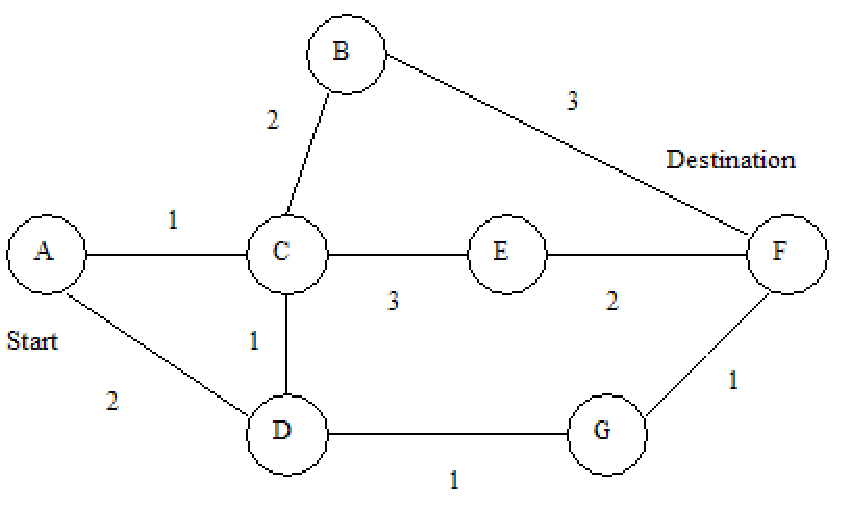
\includegraphics[width=5cm]{../img/dijkstras-graph.pdf}
\end{center}
\begin{tabular}{ll}
  \hh{Nodes} & $($ \w{fact}, truth maintained $\in\{\textrm{true}, \textrm{false}\})$ \\
  & \\
  \pause
  \hh{Start Node} & $($ \w{query fact}, \true{true} $)$ \\
  \hh{End Nodes}  & \w{any known fact} \\
  & \\
  \pause
  \hh{Edges} & Mutations of the current fact \\
  \pause
  \hh{Edge Costs} & How ``wrong'' an inference step is (learned) \\
\end{tabular}
\end{frame}

%%%%%%%%%%%%%%%%%% 
% EXAMPLE SEARCH
%%%%%%%%%%%%%%%%%%
\input exampleSearch.tex

%%%%%%%%%%%%%%%%%%%% 
%% EDGE TEMPLATES
%%%%%%%%%%%%%%%%%%%%
%\begin{frame}{Edge Templates}
%\begin{center}
%  \begin{tabular}{p{0.4\textwidth}p{0.20\textwidth}}
%    \multicolumn{1}{c}{\textbf{Template}} & \multicolumn{1}{c}{\textbf{Instance}} \\
%    Hypernym & \w{animal} $\rightarrow$ \w{cat} \\
%    Hyponym  & \w{cat} $\rightarrow$ \w{animal} \\
%    Antonym  & \w{good} $\rightarrow$ \w{bad} \\
%    Synonym  & \w{cat} $\rightarrow$ \w{true cat} \\
%    & \\
%    Add Word  & \w{cat} $\rightarrow$ \w{$\cdot$} \\
%    Delete Word  & $\cdot$ $\rightarrow$ \w{cat} \\
%    & \\
%    Operator Weaken & \w{some} $\rightarrow$ \w{all} \\
%    Operator Strengthen & \w{all} $\rightarrow$ \w{some} \\
%    Operator Negate & \w{all} $\rightarrow$ \w{no} \\
%    Operator Synonym & \w{all} $\rightarrow$ \w{every} \\
%    & \\
%    Nearest Neighbor  & \w{cat} $\rightarrow$ \w{dog} \\
%  \end{tabular}
%\end{center}
%\end{frame}


%%%%%%%%%%%%%%%%%%%% 
%% DELETIONS (INSERTIONS)
%%%%%%%%%%%%%%%%%%%%
%\begin{frame}{Inserting Words During Search}
%\begin{center}
%  \scalebox{0.8}{\wordthe \cat \eat \mice}
%\end{center}
%\end{frame}
%
%\begin{frame}[noframenumbering]{Inserting Words During Search}
%\begin{center}
%  \scalebox{0.8}{\wordthe \cat \eat \worda \mice}
%\end{center}
%\end{frame}
%
%\def\worda{\monoUpR{}{???}{}{}}
%\begin{frame}[noframenumbering]{Inserting Words During Search}
%\begin{center}
%  \scalebox{0.8}{\wordthe \cat \eat \worda \mice} \\
%  \vspace{0.5cm}
%  \exampleInsertions
%\end{center}
%\end{frame}
%
%%%%%%%%%%%%%%%%%%%% 
%% STORE FACTS AS A TRIE
%%%%%%%%%%%%%%%%%%%%
%\def\title{Store Facts as a Trie}
%\begin{frame}{\title}
%  \factTrie{dotpath}{dotpath}{dotpath}
%\end{frame}
%
%\begin{frame}[noframenumbering]{\title}
%  \factTrie{goodPath}{dotpath}{dotpath}
%\end{frame}
%
%\begin{frame}[noframenumbering]{Inserting Words During Search}
%\begin{center}
%  \scalebox{0.8}{\wordthe \cat \eat \worda \mice}
%\end{center}
%\end{frame}
%
%\def\worda{\monoUpR{}{catnip}{herb}{tracheophyte}}
%\begin{frame}[noframenumbering]{Inserting Words During Search}
%\begin{center}
%  \scalebox{0.8}{\wordthe \cat \eat \worda \mice}
%\end{center}
%\end{frame}
%
%\begin{frame}[noframenumbering]{\title}
%  \factTrie{dotpath}{goodPath}{dotpath}
%\end{frame}
%
%\def\worda{\monoUpR{}{???}{}{}}
%\begin{frame}[noframenumbering]{Inserting Words During Search}
%\begin{center}
%  \scalebox{0.8}{\wordthe \cat \eat \worda \mice}
%\end{center}
%\end{frame}
%
%\def\worda{\monoUpR{}{my}{}{}}
%\begin{frame}[noframenumbering]{Inserting Words During Search}
%\begin{center}
%  \scalebox{0.8}{\wordthe \cat \eat \worda \mice}
%\end{center}
%\end{frame}
%
%\begin{frame}[noframenumbering]{\title}
%  \factTrie{dotpath}{dotpath}{goodPath}
%\end{frame}
%
%\def\worda{\monoUpR{}{???}{}{}}
%\begin{frame}[noframenumbering]{Inserting Words During Search}
%\begin{center}
%  \scalebox{0.8}{\wordthe \cat \eat \worda \mice}
%\end{center}
%\end{frame}
%
%\def\worda{\monoUpR{\textbf{All$_{\downarrow \uparrow}$}}{\darkgreen{\textbf{a$_{\uparrow \uparrow}$}}}{}{}}
%\begin{frame}[noframenumbering]{Inserting Words During Search}
%\begin{center}
%  \scalebox{0.8}{\wordthe \cat \eat \worda \mice}
%\end{center}
%\end{frame}


%%%%%%%%%%%%%%%%%%% 
% SOFT LOGIC
%%%%%%%%%%%%%%%%%%%
\begin{frame}{``Soft'' Natural Logic}
\hh{Want to make likely (but not certain) inferences}.
\begin{itemize}
  \item Same motivation as Markov Logic, Probabilistic Soft Logic, etc.
  \pause
  \item Each \textit{edge template} has a cost $\theta \geq 0$.
\end{itemize}
\vspace{0.5cm}
\pause

\hh{Detail:} Variation among \textit{edge instances} of a template.
\begin{itemize}
  \item WordNet: \w{cat} $\rightarrow$ \w{feline} \textbf{vs.} \w{cup} $\rightarrow$ \w{container}.
  \item Nearest neighbors distance.
  \item Each \textit{edge instance} has a distance $f$.
\end{itemize}
\vspace{0.5cm}
\pause

\begin{tabular}{ll}
\hh{Cost of an edge is} & $\theta_i \cdot f_i$. \\
\pause
\hh{Cost of a path is} & $\theta \cdot \mathbf{f}$. \pause \\
\multicolumn{2}{l}{\hh{Can learn parameters $\theta$}.}
\end{tabular}

\end{frame}

%%%%%%%%%%%%%%%%%%% 
% CONCLUSION
%%%%%%%%%%%%%%%%%%%
\begin{frame}{Summary: NaturalLI}
\hh{High-Level Takeaways}
\begin{itemize}
  \item \textit{Deep} inferences from a \textit{large} knowledge base.
  \item Leverage arbitrarily large plain-text knowledge bases.
  \item ``Soft'' logic with probability of truth.
\end{itemize}
\vspace{0.5cm}
\pause

\hh{Results}
\begin{itemize}
  \item ConceptNet facts: 12\% recall $\rightarrow$ 49\% recall @ 91\% precision.
  \item Checks logical entailment (not just fuzzy query).
\end{itemize}
\vspace{0.25cm}
\pause

\hh{Complexity doesn't grow with knowledge base size.}
\end{frame}
